\begin{figure*}[t]
\centering
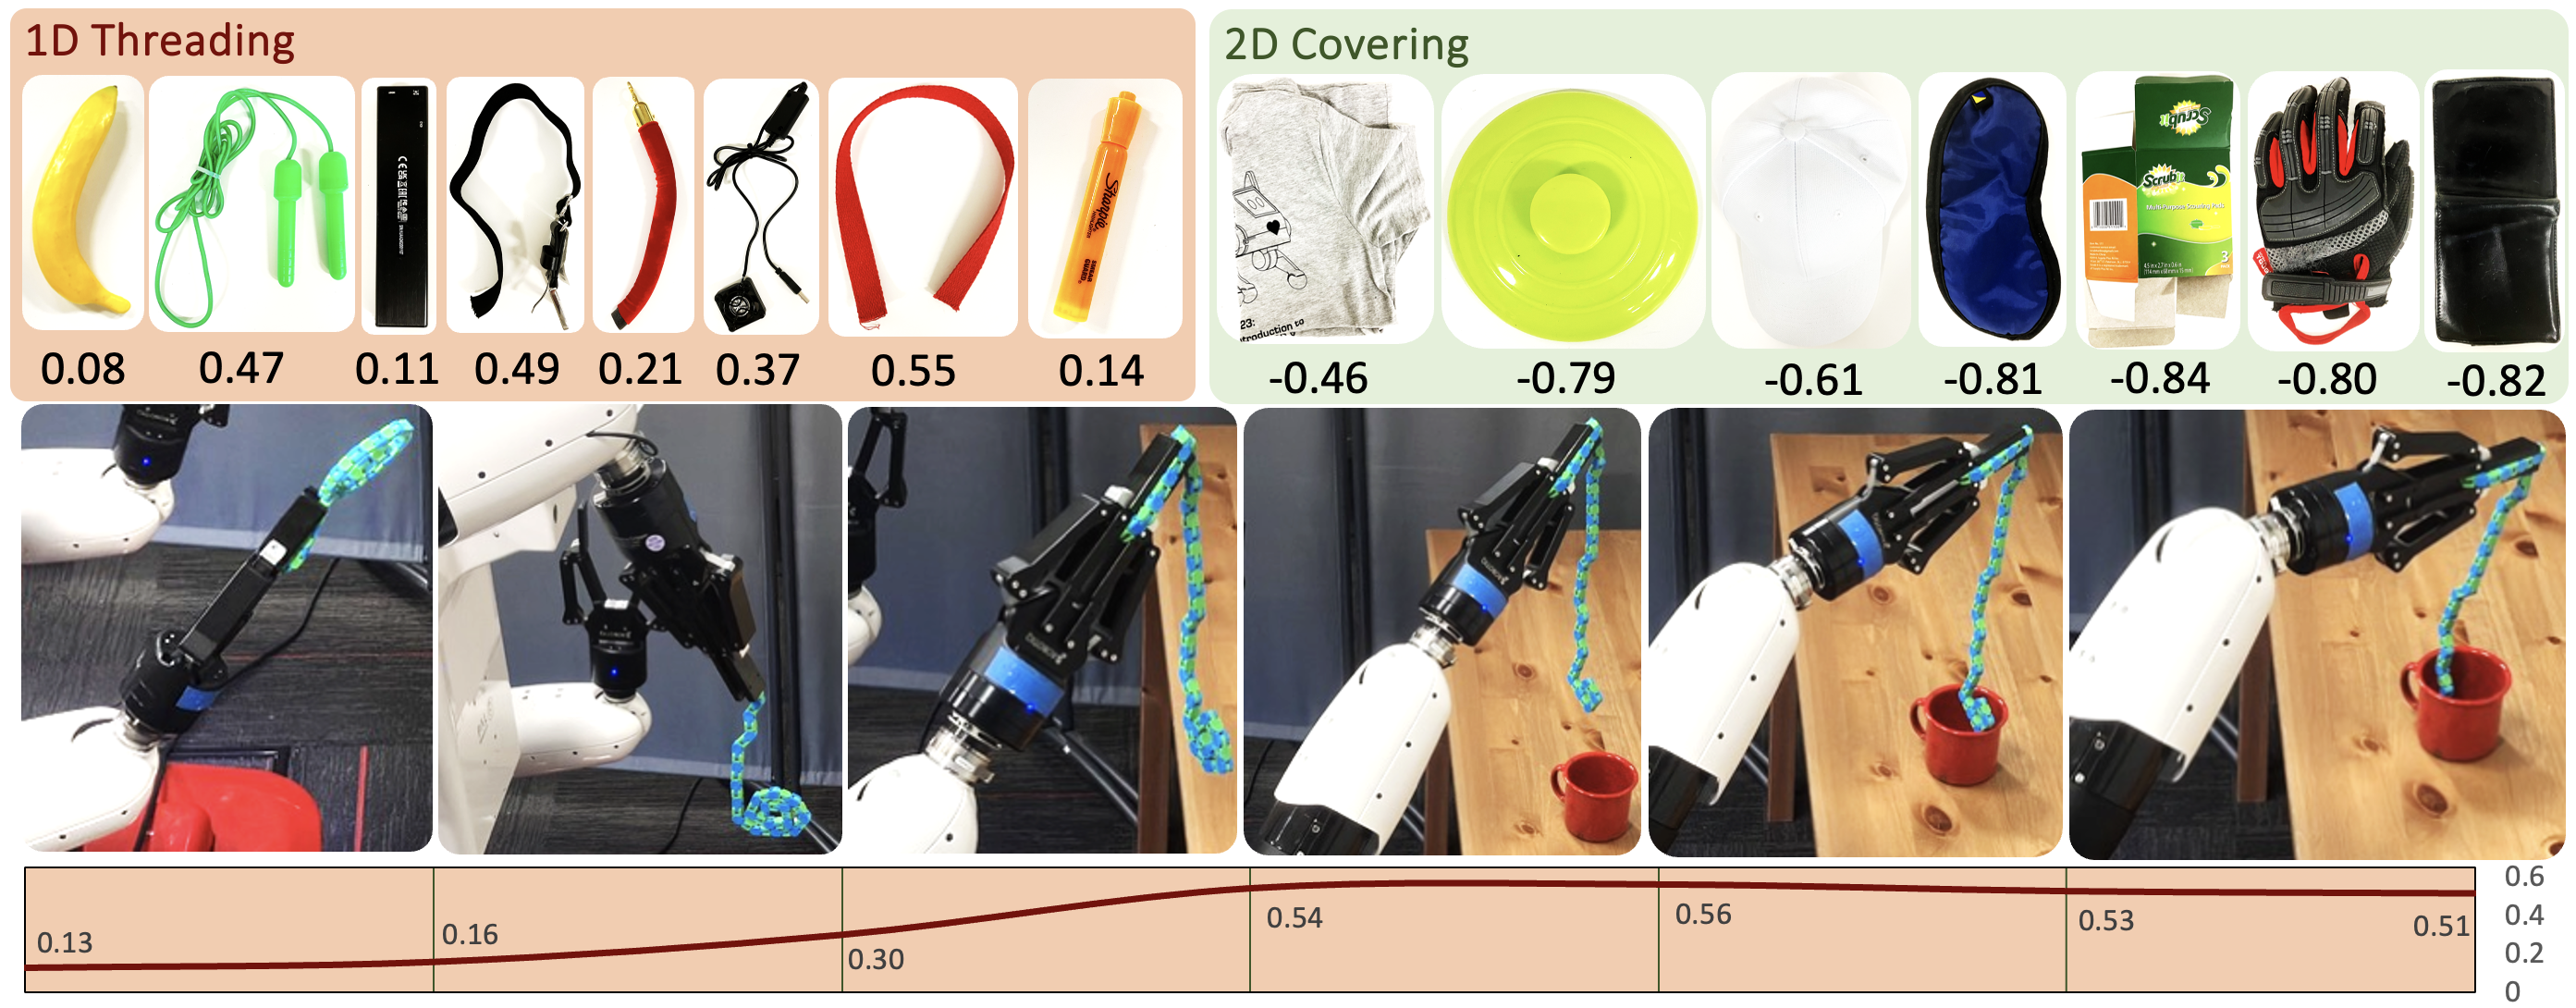
\includegraphics[width=\linewidth]{photos/embedding.png}
\caption{\textbf{Visualization of \methodname{}'s dynamics embedding} in \taskone~(\textcolor{Orange}{\textit{Top-Left}}) and \tasktwo~(\textcolor{OliveGreen}{\textit{Top-Right}}) tasks. The number below each object photo is the value of a single dimension of the dynamics embedding. \textcolor{Orange}{\textit{Bottom}}: the rollout of the policy given a special object whose rigidity changes with rotation. The line charts below the rollout visualize the value of a single dimension of the dynamics embedding during robot execution. We see that certain dimensions of the dynamics embedding are strongly correlated with the softness of the objects, demonstrating the adaptation module's ability to infer the softness of the objects. }
\label{fig:embedding}
\end{figure*}
\section{Experiments}
\label{sec:experiments}
In our experiments, we use a TIAGo robot (Fig.~\ref{fig:tasks}), which is a 22-DOF bimanual mobile manipulator with 3-DOF for the omnidirectional base, 7-DOF for each of the two arms, 1-DOF torso, 2-DOF head, and 1-DOF for each of the two Robotiq parallel-jaw grippers. The robot has an RGB-D camera mounted on its head. 
We use depth images of $224 \times 224$ resolution captured at 3 Hz. 
In both simulation and the real world, \methodname{}'s input is the robot's depth image and joint angles.

We use OmniGibson~\cite{li2023behavior, li2024behavior} as the training simulator for \methodname{}. In OmniGibson, A model of the same TIAGo robot is placed in front of a simulated version of the task (Fig.~\ref{fig:tasks}). To train the visuomotor mobile manipulation policy, we use a binary reward of 1 for task success and a small reward negatively correlated with the distance between the deformable object and the target rigid-body object on the table.
In the real world, the robot is placed in front of an unseen table with unseen deformable and rigid-body objects (Fig.~\ref{fig:tasks}). 
\methodname{} then controls the robot's bimanual mobile manipulation capabilities (base, torso, head, grippers, and arms) to grasp and manipulate the deformable object to achieve the task, using all DOFs simultaneously.
All experiments are conducted autonomously without human intervention from raw visual inputs with no QR codes. 
We use real-world objects (Fig.~\ref{fig:objects}), environments (Fig.~\ref{fig:tasks}), and lighting conditions (Fig.~\ref{fig:tasks}) never seen during simulation training. 
We repeat each task 20 times with different initial locations and objects. 

\textbf{Tasks}: We evaluate \methodname{} across two challenging deformable-object mobile manipulation tasks that require online adaptation to the deformable object's unknown dynamics a priori: \taskone~and \tasktwo. In \taskone~(Fig.~\ref{fig:tasks}, \textit{left}), the goal is to pick up a 1D deformable object on the table and insert either one of its two ends into a container. In the real-world version of the task, we place a 1D deformable object randomly on the table, selected across 20 categories such as rope, cables, and belts~(Fig.~\ref{fig:objects}, \textit{left}), and a container selected across 20 object categories such as cups, bowls, and pans. Success is defined by whether the robot inserts one end of the deformable object into the container within 300 seconds. 
In \tasktwo~(Fig.~\ref{fig:tasks}, \textit{right}), the goal is to pick up a 2D deformable object on the table and cover the opening of a container on the table-- a representative task in household scenarios. In the real-world version of the task, we place a 2D deformable object randomly on the table, sampled across 20 categories such as lids, napkins, towels, and plastic films~(Fig.~\ref{fig:objects}, \textit{right}). There is no parameter randomization applied to object pose, material stiffness, or friction, since such randomization is achieved implicitly via object instance randomization. Success is defined by whether the robot successfully covers 90\% of the container's opening within 300 seconds. 
Achieving both tasks requires closed-loop hand-eye coordination, robustness against object deformation and occlusions, and online adaptation to the unknown dynamics of the deformable object during real-time interaction, as shown in Fig.~\ref{fig:rollout} and \ref{fig:embedding}.

\begin{table*}[t]
\centering
\small
\caption{\textbf{Successful Trials} Out of 20 and Success Rates for \methodname{}, Baselines and Ablations}
\label{tab:results}
\resizebox{\linewidth}{!}{
\begin{tabular}{|c|c|c|c|c|c|c|c|}
\toprule
 & \methodname{} & DMfD & DDOD & \methodname{}-No-Adapt & a\methodname{}-No-Shape & \methodname{}-E2E \\
\midrule
\taskone & 17 (85\%) & 3 (15\%) & 2 (10\%) & 7 (35\%) & 7 (35\%) & 5 (25\%) \\ 
\tasktwo & 16 (80\%) & 1 (5\%)  & 5 (25\%) & 5 (25\%) & 9 (45\%) & 4 (20\%) \\\midrule
Total & 33 / 40 (82.5\%) & 4 / 40 (10\%) & 7 / 40 (17.5\%) & 12 / 40 (30\%) & 16 / 40 (40\%) &  9 / 40 (22.5\%)\\
\bottomrule
\end{tabular}}
\end{table*}
\textbf{Baselines}: We compare \methodname{} to two baselines for learning deformable object manipulation: DMfD~\cite{salhotra2022learning} (Table~\ref{tab:results}, \textit{column 3}) and DDOD~\cite{sundaresan2020learning,ganapathi2021learning} (Table~\ref{tab:results}, \textit{column 4}). The first baseline, DMfD, learns deformable object stationary manipulation of 1D and 2D object categories from simulated expert demonstrations. The second baseline, DDOD, learns dense object descriptor representations for 1D~\cite{sundaresan2020learning} and 2D~\cite{ganapathi2021learning} deformable objects and learns deformable object stationary manipulation from a single human demonstration using this representation. To make DDOD comparable to \methodname{}, which requires no demonstrations, we script a policy based on the dense object descriptors learned from DDOD to perform deformable object manipulation, instead of providing human demonstrations. To help both baselines overcome failures in grasping the deformable object and acquire navigation capabilities comparable to \methodname{}, we use \methodname{} to execute the grasping and navigation of the tasks before activating the baseline for the deformable object manipulation part of the tasks. Learning deformable object mobile manipulation with unseen deformable object dynamics, categories, and instances using real-robot imitation learning~\cite{black2024pi0,kim2024openvla,team2024octo,zhao2024aloha,zhao2023learning,nair2017combining,brohan2023rt,brohan2022rt,liu2024rdt} requires collecting an infeasible number of real-world demonstrations on the TIAGo robot, which makes them incomparable to \methodname{}, since \methodname{} requires no real-robot demonstrations. Extending \methodname{} to fine-tune on real-world data to compare to these methods is left for future work.

We also conduct three ablation experiments of \methodname{}: 1) \textit{\methodname{}-\textit{No-Adapt}} (Table~\ref{tab:results}, \textit{column 5}), which removes both the Shape and Dynamics Adaptation Modules and trains \methodname{}'s visuomotor policy only; 2) \textit{a\methodname{}-No-Shape} (Table~\ref{tab:results}, \textit{column 6}), which deletes the Shape Adaptation Module and trains only the visuomotor policy and the Dynamics Adaptation module; and 3) \textit{\methodname{}-E2E} (Table~\ref{tab:results}, \textit{column 7}), which ignores both Shape and Dynamics Encoders, skips the first of the two training phases and trains \methodname{} with end-to-end RL without the two L1 losses.

In our experiments, we answer four main questions:

\textbf{Q1: How does \methodname{} compare to state-of-the-art sim2real methods in real-robot deformable object mobile manipulation?} In Table~\ref{tab:results} (columns 2-4), \methodname{} outperforms both baselines significantly across both tasks. Qualitatively, DMfD fails in both \taskone~and \tasktwo~because after grasping, the deformable object suffers from severe deformation and occlusions by the robot gripper during the hand-eye-coordinated motions of inserting and covering, preventing DMfD from generating a sufficiently accurate segmentation mask for the deformable object. In some cases where the segmentation mask is accurate enough, DMfD is still unable to adapt to the unknown dynamics of the deformable object. DDOD fails in \taskone~and \tasktwo~because the deformable object suffers from in-the-wild, non-top-down camera viewpoints, severe deformation, and robot gripper occlusions, making DDOD incapable of predicting accurate dense object descriptors for the deformable object during manipulation.
In some cases where the dense object descriptor predictor performs well, DDOD is still unable to adapt to the unknown dynamics of the deformable object. In contrast, \methodname{} performs closed-loop 6-DOF control and hand-eye coordination directly from non-top-down depth images and outperforms both DMfD and DDOD. 

\textbf{Q2: How important are \methodname{}'s Shape and Dynamics Adaptation Modules to deformable object mobile manipulation?} We compare \methodname{} (Table~\ref{tab:results}, \textit{column 2}) to \textit{\methodname{}-\textit{No-Adapt}} (Table~\ref{tab:results}, \textit{column 5}), which ablates Shape and Dynamics Adaptation Modules. We observe a 52.5\% drop in performance for \methodname{}-\textit{No-Adapt}. Qualitatively, in both \taskone~and \tasktwo, \methodname{}-\textit{No-Adapt} treats deformable objects as rigid objects, which fails when the object is made of soft materials. Therefore, \methodname{}'s Adaptation Modules are crucial.

\textbf{Q3: How important is \methodname{}'s ability to infer the object's shape changes?} We compare \methodname{} to \textit{a\methodname{}-No-Shape} (Table~\ref{tab:results}, \textit{column 6}), which removes the Shape Adaptation Module. We observe that \methodname{} encounters a 42.5\% success rate degradation compared to our full variant using both the Shape and Dynamics Adaptation Modules. In both \taskone~and \tasktwo, we observe that \textit{a\methodname{}-No-Shape} is successful at grasping the deformable object and moving it closer to the target container to insert or cover, but unable to execute the precise dynamic motion needed to insert or cover the container, which requires inferring the deformable object's shape changes. Thus, the ability to infer how the object's shape changes is crucial. 

\textbf{Q4: Is optimizing both adaptation modules to mimic their corresponding ground-truth encoders necessary, or is end-to-end RL sufficient for task success?} We compare \methodname{} to \textit{\methodname{}-E2E} (Table~\ref{tab:results}, \textit{column 7}), which trains the entire architecture with end-to-end RL. We observe that \textit{\methodname{}-E2E} fails to converge optimally on its RL policy gradients during training and experiences a 60\% success rate reduction: due to the high-dimensionality of the 10 most recent depth image observations and unstable RL training gradient signals, \methodname{} relies solely on current depth observations to perform the task, ignoring and failing to learn a useful dynamics embedding. Thus, optimizing both adaptation modules using L1-loss in a two-phase training process is crucial. 